\section{Experimental Design} 
\label{sec:Evaluation}

In this section we explain how we empirically evaluate our proposal for automated transplantation in video games through \ApproachName{}. Through this section, we present the research questions that we aim to answer, the evaluation process, and the implementation details.

\subsection{Research Questions}

\simhotep{} propose a new angle for PCG, and for that reason we want to compare it to the established practice in the video game field in our first research question:

\textbf{RQ$_1$: }\textit{How does \simhotep{} perform with respect to the PCG baseline?}

\simhotep is also a new angle to guide the transplantation. We propose to leverage the possibilities of the vide game domain by means of simulations, so we want to compare it to the established practice (test suite to guide the transplantation) in the software transplantation field. This motivates our second research question:

\textbf{RQ$_2$: }\textit{What is the performance in terms of solution quality of \simhotep{} and \timhotep{}?}

% \textbf{RQ$_1$: }\textit{What is the performance in terms of solution quality of \ApproachName{} with the simulation-based \ApproachName{} ($S_{Imhotep}$), \ApproachName{} with the test-based \ApproachName{} ($T_{Imhotep}$), and the PCG baseline?}

% \textbf{RQ$_2$: }\textit{Is there any difference in the quality of the solution among \ApproachName{} with the simulation-based \ApproachName{}, \ApproachName{} with the test-based \ApproachName{}, and the PCG baseline?}

% \textbf{RQ$_3$: }\textit{Are the performance results obtained by \ApproachName{} with the simulation-based \ApproachName{}, \ApproachName{} with the test-based \ApproachName{}, and the PCG baseline significant?}


\subsection{Planning and execution}

Fig.~\ref{fig:evaluation} shows an overview of the evaluation. The white background part at the top shows the assets of the game itself (content) and the game development (test suite) that are used by the approaches. The grey background part in the middle shows the inputs and outputs of the three approaches (the two \ApproachName{} variants and the baseline). Finally, the white background part at the bottom shows the evaluation of the results of the approaches.

We used the work by Gallota \etal~\cite{gallotta2022evolving} as PCG baseline. Gallota \etal proposed a hybrid Evolutionary Algorithm for generating NPCs. Specifically, their approach combines an L-system with a Feasible Infeasible Two Population Evolutionary Algorithm. We choose Gallota \etal as PCG baseline because (1) this work is specific for spaceships that can play the role of bosses which is comparable to the content of the case study, and (2) it achieves the best state-of-the-art results for that content. 

In the evaluation we also include a test-based variant of \ApproachName{} (\timhotep{}). In this variant, the assessment is carried out by passing tests. The reason for including this variant is that in classic software transplantation the best results have been achieved by using the test suite for the assessment.
For the \timhotep{} we ask the developers to provide the set of tests that are relevant for the evaluation. The developers from \CaseStudy{} provided us with a total of 243 tests selected based on their domain knowledge. The objective value will be retrieved when each individual pass through the 243 tests, normalized in a scale of [0, 1]. An individual which passes the 243 tests will obtain 1.0, on the contrary if it does not pass any test it will obtain 0.0. As in the \simhotep{}, the each individual needs to pass through a validation, giving 0.0 to those that are not valid.

For the evaluation we used five different hosts (Vermis, Teuthus, Argos, Orion, and Maia), which are the full set of original bosses from the video game \CaseStudy{}. As donors, \CaseStudy{} developers considered all \CaseStudy{}'s scenarios to identify 129 organs. Each host has more than a thousand model elements. Organs have an average of 255 model elements.

Each organ was transplanted individually to each boss. Each variant of \ApproachName{} provided a total of 645 new individuals (5 hosts * 129 organs) as output, 645 new individuals from \simhotep{} and 645 individuals from \timhotep{}. In the case of the baseline (which relies on the L-system to generate the content instead of transplanting organs), to make it a fair comparison, the baseline was executed 129 times with each one of the 5 different hosts to obtain 645 new individuals. In addition, we executed 30 independent runs (to account for random variation as suggested by Arcuri and Fraser~\cite{arcuri2013parameter}). Hence, we obtain a total of 58050 independent runs (645*3*30).

To compare the solutions of the baseline and the two variants of \ApproachName{} (\simhotep{} and \timhotep{}), we rely on the concept of game quality and its automated measurement through simulated players. The results of Browne \etal demonstrated the validity of the approach which is widely accepted in the research community~\cite{browne2010evolutionary}. Therefore, we need two ingredients to run our experiment: The simulated player and the automated measurement.

The simulated player, developed by the developers of the \CaseStudy{} video game, possesses the ability to mimic human player behaviour. Our approach incorporates their algorithm, utilizing it to simulate battles between the generated bosses and the simulated player. Within these simulations, the simulated player confronts the boss, strategically targeting and destroying its weak points. Meanwhile, the boss operates in accordance with its anatomical structure, behavioural patterns, and attack/defensive dynamics, aiming to overcome the simulated player. Both entities within the simulation actively strive to emerge victorious, eschewing draws or ties, and ensuring a definitive win. The algorithm grants the simulated player the capability to employ various strategies when engaging with a boss, as it can be parameterized to define its fighting approach. The simulation parameters were provided by the developers, who analysed battles between human players and bosses to inform their decision-making.

The automated measurement is $Q_{Duration}$ which was proven to achieve good results~\cite{browne2010evolutionary}. The duration of duels between simulated players and bosses units is expected to be around a certain optimal value. For the \CaseStudy{} case study, through tests and questionnaires with players, the developers determined that concentration and engagement for an average boss reach their peak at approximately 10 minutes ($T_{Optimal}$), whereas the maximum accepted time was estimated to be 20 minutes ($2*T_{Optimal}$). Significant deviations from that reference value are good design-flaw indicators: short games are probably too easy; and duels that go on a lot longer than expected tend to make players lose interest. The criterion $Q_{Duration}$ is a measure of the average difference between the duration of each duel ($T_{d}$) and the desired, optimal duration ($T_{Optimal}$):
\begin{equation}
Q_{Duration} =  1 - \frac{\sum\limits_{d=1}^{Duels}\frac{\mid T_{Optimal} - T_{d} \mid}{T_{Optimal}}}{Duels} 
\end{equation}

\begin{figure}[h]
    \centering
    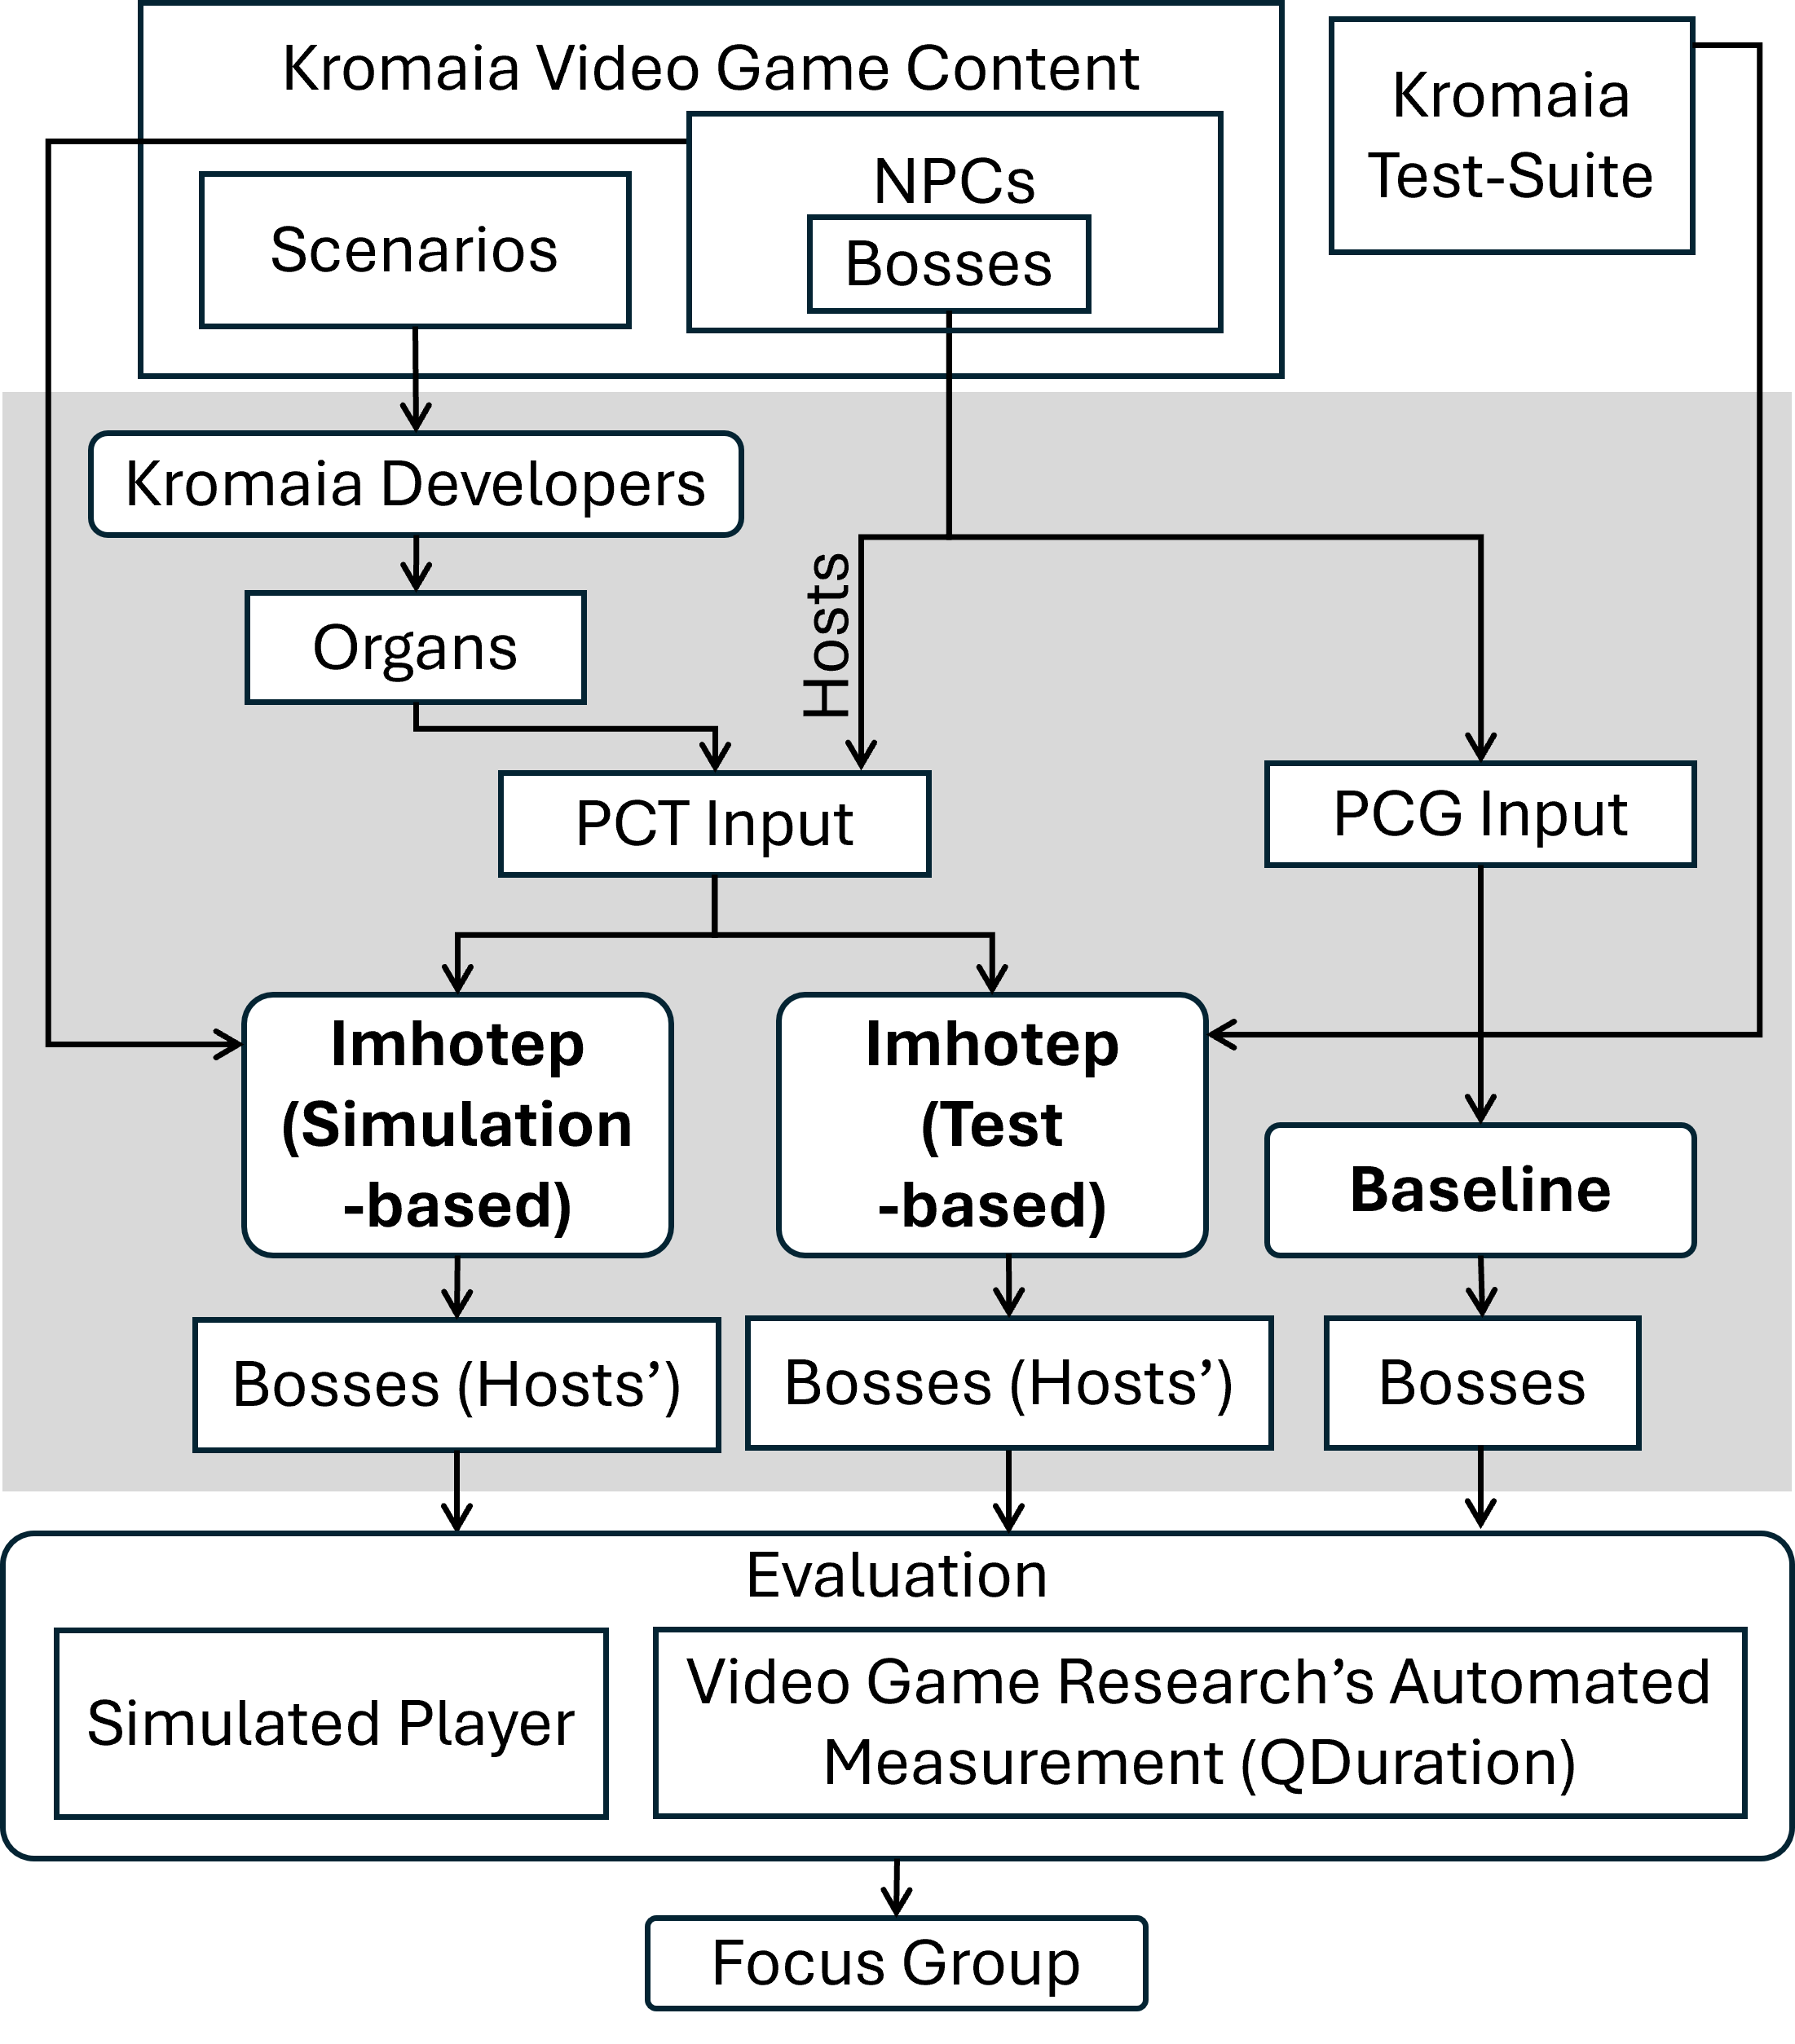
\includegraphics[width=0.4\textwidth]{Figures/evaluation_process.png}
    \caption{Overview of the evaluation process.}
    \label{fig:evaluation}
\end{figure}

\subsection{Implementation details}

We chose the parameters shown in Table~\ref{tab:evaluation_parameters} to calibrate our \ApproachName{} approach. We established the stop condition at 2 minutes and 30 seconds, ensuring that the approaches run long enough to obtain suitable solutions. The focus of this paper is not to tune the values to improve the performance of the approaches when applied to a specific problem, but rather to compare the performance of the approaches in terms of solution quality on a level playing field.

The evaluation of \ApproachName{} and the baseline was done using two PCs with the following specifications; Intel Core i7-8750H, 16GB; and  2x Intel(R) Xeon(R) CPU X5660, 64GB.
The implementation uses the Java(TM) SE Runtime Environment (JDK 1.8), together with Java as the programming language. 
For purposes of replicability and extension of our work, the implementation source code and the data are publicly available at the following URL: \url{https://anonymous.4open.science/r/Imhotep/}

\begin{table}[h]
    \centering    
    \caption{\ApproachName{} parameter settings}
    \begin{tabular}{ll}
        \hline
        \bf{Parameter description}            & \bf{Value}  \\ \hline
        Stop Criterion                   & 2m 30s \\
        Population size                  & 100    \\
        Number of parents                & 2      \\
        Number of offspring              & 2      \\
        Crossover probability            & 1      \\
        Mutation probability             & 1/150 \\ \hline
    \end{tabular}

    \label{tab:evaluation_parameters}
    \end{table}

% \subsection{Quality measurements}
% \label{subsec:Measurements}

% In a recent research done by Browne et al., the experimentation with game users showed that the following criteria stand out as being the most important: Completion, Duration, Uncertainty, Killer Moves, Permanence, and Lead Change \cite{browne2010evolutionary}. Our evaluation measures these criteria with values in the interval [0,1].

% {\bf Completion (Viability):} A game against a boss unit should end with more conclusions (victories for either the player or the boss) than draws/ties. The criterion $Q_{Completion}$ calculates a ratio of conclusions over total duel count:
% \begin{equation}
% Q_{Completion} = \frac{Conclusions}{Duels}
% \end{equation}

%  {\bf Uncertainty (Quality):} In order to keep players engaged with a duel, neither the player nor the boss unit should get extremely close to victory or defeat too early before the duel is settled, with ($T_{d}$) being its duration. Therefore, a duel is considered to be more uncertain the longer the time until the player's or the boss unit's health levels reach a dangerous/critical status ($P_{d}$ and $B_{d}$, respectively). For each duel, $Q_{Uncertainty}$ measures the average deviation between the time at which it is detected that one of the contenders is on the verge of defeat and the time corresponding to the duration of the duel.
% \begin{equation}
% Q_{Uncertainty} =  1 - \frac{\sum\limits_{d=1}^{Duels}\frac{T_{d} - min\left ( P_{d}, B_{d} \right )}{T_{d}}}{Duels} 
% \end{equation}

% {\bf Killer Moves:}   $Q_{KMoves}$ measures the proportion of killer moves by any contender ($K$), taking into account the moves that are considered to be remarkable highlights ($H$) but that are less important than killer moves. In the video game case study, the developers considered that a highlight move happens when either the boss unit or the player experiences a decrease in health; killer moves are those that make the difference in health between the contenders reach 30\%.
% \begin{equation}
% Q_{KMoves} =  1 - \frac{\sum\limits_{d=1}^{Duels}\frac{K_{d}}{H_{d}}}{Duels} 
% \end{equation}

% {\bf Permanence:} Duels with a high permanence value are games in which the advantages given by significant actions or moves by one of the contenders are unlikely to be immediately reverted by the opponent in terms of dominance. In the video game case study, the developers considered every highlight move and killer move to be meaningful actions, with recovery moves ($R$) being those that quickly cancelled the advantages given by other previous killer or highlight moves. The criterion $Q_{Permanence}$ is measured as follows:
% \begin{equation}
% Q_{Permanence} =  1 - \frac{\sum\limits_{d=1}^{Duels}\frac{R_{d}}{H_{d}+K_{d}}}{Duels} 
% \end{equation}

% {\bf Lead Change:} The lack of lead changes indicates low dramatic value. In the video game case study, the lead is determined at any given moment by considering the contender with the highest health level. This criterion is measured taking into account those highlight or killer moves that cause the lead to change ($L$) during the course of a duel:
% \begin{equation}
% Q_{LChange} = \frac{\sum\limits_{d=1}^{Duels}\frac{L_{d}}{H_{d}+K_{d}}}{Duels} 
% \end{equation}

% $Q_{Overall}$ calculates an average quality value for a model, including all of the quality criterion studied:
% \begin{equation}
% Q_{Overall} = \frac{\sum\limits_{i=1}^{N}Q_{i}}{N}
% \end{equation}